\documentclass[11pt]{article}
\usepackage[margin=1in]{geometry}
\usepackage{amsmath,amssymb}
\usepackage{enumitem}
\usepackage{xcolor}
\usepackage{url}
\usepackage{wrapfig} 
\usepackage{needspace}
\usepackage[normalem]{ulem}
\usepackage[font=small, labelfont={bf,color=navy}, justification=centering]{caption}
\definecolor{navy}{RGB}{20,30,110}
\setlist{itemsep=1pt, topsep=3pt}
\newcommand{\head}[1]{\needspace{5\baselineskip}\vspace{0.5em}\noindent{\large\bfseries\color{navy}\uline{#1}}\par\vspace{0.15em}}
\newcommand{\subhead}[1]{\vspace{0.4em}\noindent{\bfseries\color{navy}#1}\par\vspace{0.1em}}
\newcommand{\runin}[1]{{\bfseries\color{navy}#1}\enspace}
\newcommand{\note}[1]{\\[-0.2em]{\small\color{black!70}#1}}
% Parameter table: Parameter | Dim. | Source | Method | Value / range
\newenvironment{ptable}
  {\par\smallskip\noindent\small
   \begin{tabular}{@{}p{1.9cm} p{1.2cm} p{3.6cm} p{4.5cm} p{3.7cm}@{}}
   \hline
   \textbf{Parameter} & \textbf{Dim.} & \textbf{Source} & \textbf{Method} & \textbf{Value / range} \\
   \hline}
  {\hline\end{tabular}\par\smallskip}
% Numbered assumptions (A1, A2, ...) continue across sections
\newlist{assume}{enumerate}{1}
\setlist[assume]{label=\textbf{A\arabic*.}, ref=A\arabic*, leftmargin=1cm, noitemsep}
\usepackage{tikz}
\usetikzlibrary{arrows.meta, shapes.geometric, calc}

\begin{document}

\begin{center}
  {\large IEOR E4004 Optimization Models and Methods, Section 001}\\[0.2em]
  {\Large\bfseries\color{navy} Milestone 4: Complete Optimization Model}\\[0.2em]
  {\itshape Optimization for a Northeast Corridor Natural Gas Merchant}\\[0.2em]
  Team 23 (L) \quad\textbullet\quad November 4, 2026
\end{center}

\head{Summary}
A natural gas merchant, modeled on BP's U.S.\ gas marketing business, buys gas at a western
Pennsylvania hub and ships it on firm pipeline capacity to contracted customers in New York, New
Jersey, and eastern Pennsylvania. It leases storage at the hub and in New York, and can also buy gas
at each market's delivered (citygate) price. A multi-period linear program chooses monthly purchases,
storage operations, shipments, spot purchases, and firm capacity over the storage year (April 2025 --
March 2026) to meet demand at minimum cost. The core trade-off is how to cover winter demand: firm
pipeline capacity, summer fills of market-area storage, or winter spot purchases.

\head{Sets}
\vspace{-0.4\baselineskip}
\begin{itemize}[leftmargin=1cm, noitemsep, label=--]
  \item $T = \{1,\dots,12\}$: months, April 2025 ($t=1$) through March 2026 ($t=12$)
  \item $J = \{\mathrm{NY}, \mathrm{NJ}, \mathrm{PA}\}$: delivery markets
  \item $L = \{1,2,3,4\}$: firm pipeline routes from the hub; $L_j \subseteq L$ are the routes into
        market $j$: $L_{\mathrm{NY}} = \{1,2\}$, $L_{\mathrm{NJ}} = \{3\}$, $L_{\mathrm{PA}} = \{4\}$
  \item $F = \{H, M\}$: leased storage fields at the hub ($F_0 = \{H\}$) and in New York
        ($F_{\mathrm{NY}} = \{M\}$; $F_{\mathrm{NJ}} = F_{\mathrm{PA}} = \emptyset$)
\end{itemize}

\head{Decision Variables}
\vspace{-0.4\baselineskip}
\begin{itemize}[leftmargin=1cm, noitemsep, label=--]
  \item $x_t$: gas purchased at the hub in month $t$ (Dth)
  \item $q^{\mathrm{in}}_{f,t},\ q^{\mathrm{out}}_{f,t}$: gas injected into and withdrawn from field $f$ in month $t$ (Dth)
  \item $I_{f,t}$: inventory in field $f$ at the end of month $t$ (Dth)
  \item $s_{\ell,t}$: gas shipped on route $\ell$ in month $t$, measured at the hub (Dth)
  \item $u_{j,t}$: gas bought at the citygate price in market $j$ in month $t$ (Dth)
  \item $k_\ell$: firm capacity contracted on route $\ell$ (Dth/day)
\end{itemize}
All decision variables are continuous and non-negative.

\begin{figure}[h!]
\centering
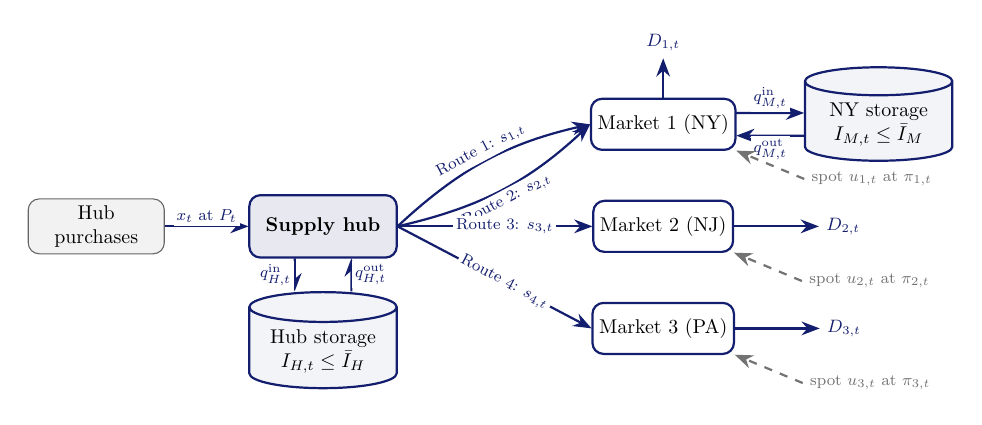
\begin{tikzpicture}[
scale=0.72, transform shape,
  >=Stealth,
  hub/.style={draw=navy, fill=navy!10, thick, rounded corners,
              minimum width=2.6cm, minimum height=1.1cm, align=center},
  mkt/.style={draw=navy, fill=white, thick, rounded corners,
              minimum width=2.4cm, minimum height=0.9cm, align=center},
  src/.style={draw=black!60, fill=black!5, rounded corners,
              minimum width=2.4cm, minimum height=0.9cm, align=center},
  stor/.style={draw=navy, fill=navy!5, thick, cylinder, shape border rotate=90,
               aspect=0.25, minimum width=2.6cm, minimum height=1.1cm, align=center},
  flow/.style={->, thick, navy},
  spot/.style={->, thick, dashed, black!55},
  lbl/.style={font=\footnotesize, fill=white, inner sep=1.5pt}
]
\node[src]  (sup)   at (0,0)     {Hub\\purchases};
\node[hub]  (hub)   at (4,0)     {\bfseries Supply hub};
\node[stor] (storH) at (4,-2.2)  {Hub storage\\$I_{H,t} \le \bar{I}_H$};
\node[mkt]  (m1)    at (10,1.8)  {Market 1 (NY)};
\node[mkt]  (m2)    at (10,0)    {Market 2 (NJ)};
\node[mkt]  (m3)    at (10,-1.8) {Market 3 (PA)};
\node[stor] (storM) at (13.8,1.8) {NY storage\\$I_{M,t} \le \bar{I}_M$};
\draw[flow] (sup) -- node[lbl, above] {$x_t$ at $P_t$} (hub);
\draw[flow] ([xshift=-5mm]hub.south) -- node[lbl, left]  {$q^{\mathrm{in}}_{H,t}$} ([xshift=-5mm]storH.north);
\draw[flow] ([xshift=5mm]storH.north) -- node[lbl, right] {$q^{\mathrm{out}}_{H,t}$} ([xshift=5mm]hub.south);
\draw[flow] ([yshift=2mm]m1.east) -- node[lbl, above] {$q^{\mathrm{in}}_{M,t}$} ([yshift=2mm]storM.west);
\draw[flow] ([yshift=-2mm]storM.west) -- node[lbl, below] {$q^{\mathrm{out}}_{M,t}$} ([yshift=-2mm]m1.east);
\draw[flow] (hub.east) to[bend left=15] node[lbl, sloped, above] {Route 1: $s_{1,t}$} (m1.west);
\draw[flow] (hub.east) to[bend right=15] node[lbl, sloped, below] {Route 2: $s_{2,t}$} (m1.west);
\draw[flow] (hub.east) -- node[lbl, pos=0.55] {Route 3: $s_{3,t}$} (m2.west);
\draw[flow] (hub.east) -- node[lbl, sloped, pos=0.55] {Route 4: $s_{4,t}$} (m3.west);
\draw[flow] (m1.north) -- ++(0,0.7) node[above, font=\small] {$D_{1,t}$};
\foreach \j in {2,3} {
  \draw[flow] (m\j.east) -- ++(1.5,0) node[right, font=\small] {$D_{\j,t}$};
}
\foreach \j in {1,2,3} {
  \draw[spot] ($(m\j.south east)+(1.2,-0.5)$)
        node[right, font=\footnotesize] {spot $u_{\j,t}$ at $\pi_{\j,t}$} -- (m\j.south east);
}
\end{tikzpicture}
\caption{The merchant's network. Hub purchases and hub-storage withdrawals share the four pipeline
routes; New York is served by two competing routes and a market-area storage field; every market can
also buy at its citygate price (dashed).}
\label{fig:network}
\end{figure}

\head{Objective Function}
Minimize total annual cost: hub purchases, pipeline usage, storage injection and withdrawal, spot
purchases, and pipeline reservation charges.
\[
\min\ \sum_{t\in T}\Big[P_t x_t + \sum_{\ell\in L} c_\ell s_{\ell,t}
      + \sum_{f\in F}\big(c^{\mathrm{in}}_f q^{\mathrm{in}}_{f,t} + c^{\mathrm{out}}_f q^{\mathrm{out}}_{f,t}\big)
      + \sum_{j\in J}\pi_{j,t}u_{j,t}\Big]
      + 12\sum_{\ell\in L} R_\ell k_\ell
\]
\vspace{-0.8\baselineskip}
\note{$P_t$ = hub price; $c_\ell$ = pipeline usage charge; $c^{\mathrm{in}}_f, c^{\mathrm{out}}_f$ =
storage injection and withdrawal charges; $\pi_{j,t}$ = citygate price (all \$/Dth). $R_\ell$ = monthly
reservation charge (\$ per Dth/day of capacity per month).}

\smallskip
\noindent Because customer volumes and prices are fixed by contract (\ref{a:revenue}), revenue does not
depend on these decisions, so minimizing supply cost maximizes the merchant's margin.

\head{Constraints}
\vspace{-0.4\baselineskip}
\begin{enumerate}[leftmargin=1cm, label=--]
  \item \textbf{(HB) Hub balance.} Hub purchases plus net withdrawals from hub storage are shipped
        on the pipeline routes.
  \[ x_t + \sum_{f\in F_0}\big(q^{\mathrm{out}}_{f,t} - q^{\mathrm{in}}_{f,t}\big) = \sum_{\ell\in L} s_{\ell,t} \qquad \forall\, t\in T \]

  \item \textbf{(DM) Market balance.} Pipeline deliveries net of fuel, plus net withdrawals from
        storage in the market, plus spot purchases, meet contracted demand $D_{j,t}$.
  \[ \sum_{\ell\in L_j} (1-\phi_\ell)\, s_{\ell,t}
     + \sum_{f\in F_j}\big(q^{\mathrm{out}}_{f,t} - q^{\mathrm{in}}_{f,t}\big)
     + u_{j,t} = D_{j,t} \qquad \forall\, j\in J,\ t\in T \]
  \vspace{-0.6\baselineskip}
  \note{$\phi_\ell$ = fuel retention rate (fraction of gas shipped).}
  \\[0.2em]
  {\small Gas injected into New York storage must first cross the pipeline (or be bought locally), so
  summer capacity that would otherwise sit idle can serve winter demand. Market-area storage and firm
  winter capacity are therefore partial substitutes.}

  \item \textbf{(IB) Inventory balance.} Inventory carries over, plus injections minus withdrawals.
  \[ I_{f,t} = I_{f,t-1} + q^{\mathrm{in}}_{f,t} - q^{\mathrm{out}}_{f,t} \qquad \forall\, f\in F,\ t\in T \]
  \vspace{-0.6\baselineskip}
  \note{$I_{f,0}$ = inventory at the start of April 2025.}

  \item \textbf{(PC) Pipeline capacity.} Monthly shipments cannot exceed contracted capacity, which
        cannot exceed the capacity available to the merchant.
  \[ s_{\ell,t} \le d_t\, k_\ell, \qquad k_\ell \le \bar{k}_\ell \qquad \forall\, \ell\in L,\ t\in T \]
  \vspace{-0.6\baselineskip}
  \note{$d_t$ = days in month $t$; $\bar{k}_\ell = \beta_\ell K_\ell$, where $K_\ell$ is the pipeline's
        full capacity and $\beta_\ell$ the merchant's accessible share (Dth/day).}

  \item \textbf{(SL) Storage limits.} Injection, withdrawal, and inventory stay within field limits.
  \[ q^{\mathrm{in}}_{f,t} \le d_t\, r^{\mathrm{in}}_f, \qquad
     q^{\mathrm{out}}_{f,t} \le d_t\, r^{\mathrm{out}}_f, \qquad
     I_{f,t} \le \bar{I}_f \qquad \forall\, f\in F,\ t\in T \]
  \vspace{-0.6\baselineskip}
  \note{$r^{\mathrm{in}}_f, r^{\mathrm{out}}_f$ = maximum daily injection and withdrawal (Dth/day);
        $\bar{I}_f$ = leased working-gas capacity (Dth).}

  \item \textbf{(CI) Cyclic inventory.} Each field ends the year at its starting inventory, so stored
        gas is not drawn down for free.
  \[ I_{f,12} = I_{f,0} \qquad \forall\, f\in F \]
\end{enumerate}

\head{Parameter Estimation}
All volumes are in Dth and prices in \$/Dth (1~Dth $=$ 1~MMBtu); EIA figures in Mcf are converted at
1.037~Dth/Mcf, EIA's average heat content. All inputs cover April 2025 -- March 2026, and monthly
values are stored in CSV files read by the Gurobi model.

% ---------------------------------------------------------------------------------
\subhead{Demand}
Markets are defined at the state level to match EIA's monthly delivery series~\cite{eia}. We size the
merchant against NJR Energy Services, which sold about 108.6~Bcf in FY2025~\cite{njr}, and assume a
30~Bcf Northeast book split 45\% NY, 25\% NJ, 30\% PA. Dividing by each state's annual deliveries gives
merchant shares $\alpha_j$; applying them to monthly deliveries preserves the seasonal profile.
BP Energy Company transactions in Con Edison and New Jersey Natural Gas filings~\cite{utility}
confirm the order of magnitude.
\begin{ptable}
$\alpha_j$  & $|J|$ & NJR FY2025~\cite{njr}; EIA deliveries~\cite{eia} & Assumed book $\div$ annual state deliveries & NY 0.975\%, NJ 1.046\%, PA 0.538\% \\
$D_{j,t}$   & $|J|\times 12$ & EIA monthly deliveries by state~\cite{eia} & $\alpha_j \times$ deliveries; five missing months imputed from historical year-on-year change & Total 1.68M (Sept.) -- 4.22M (Jan.) \\
\end{ptable}
\vspace{-0.3\baselineskip}
\begin{assume}[series=assumptions]
  \item \label{a:revenue}\textbf{Fixed contract revenue.} Volumes and sale prices are set by contract
        and surplus gas is not resold.
  \item \textbf{Book size is a scenario.} The 30~Bcf book and state split are assumptions, not
        reported market shares.
\end{assume}

% ---------------------------------------------------------------------------------
\subhead{Storage}
Each field is a leased share of its state's working-gas capacity~\cite{eia} (PA 426.3~Bcf for $H$, NY
125.2~Bcf for $M$), with starting inventory set by each state's March 2025 fill ratio.
\begin{ptable}
$\bar{I}_f$ & $|F|$ & EIA working-gas capacity~\cite{eia} & Leased share: 0.5\% (PA), 1.0\% (NY) & $H$ 2.21M; $M$ 1.30M \\
$I_{f,0}$ & $|F|$ & EIA inventory, Mar.\ 2025~\cite{eia} & Fill ratio $\times \bar{I}_f$ (PA 29.7\%, NY 33.6\%) & $H$ 0.66M; $M$ 0.44M \\
$c^{\mathrm{in}}_f,\ c^{\mathrm{out}}_f$ & $|F|$ & National Fuel FSS~\cite{nfgstorage} & Same benchmark fee for both fields & 0.0381 each (\$/Dth) \\
$r^{\mathrm{in}}_f,\ r^{\mathrm{out}}_f$ & $|F|$ & UGI; Crestwood; EIA~\cite{ugi,crestwood,eia} & Scaled daily rates; constant limits (Dth/day) & $H$: 12,280 / 50,054;\newline $M$: 12,983 / 25,966 (in/out) \\
\end{ptable}
Rates are scaled estimates. The common storage fee is a benchmark; additional surcharges and
inventory-dependent rate changes are omitted.
\vspace{-0.3\baselineskip}
\begin{assume}[resume=assumptions]
  \item \textbf{Leased shares are scenarios.} The 0.5\% and 1.0\% shares (3.4~Bcf, 11\% of annual
        demand) are not observed but assumed values for a the supposed firm size.
  \item \textbf{Market-area storage is stylized.} $M$ represents storage downstream of the NY
        pipeline bottleneck, accessed through utility asset management agreements.
  \item \textbf{Lease fees are sunk.} With $\bar{I}_f$ fixed, lease fees do not affect decisions.
\end{assume}

% ---------------------------------------------------------------------------------
\subhead{Prices}
The hub is Eastern Gas South (formerly Dominion South), the most liquid Appalachian pricing point.
Citygate prices with missing months (PA Aug.\ 2025 and Feb.\ 2026, NY Mar.\ 2026) are linearly
interpolated.
\begin{ptable}
$P_t$ & 12 & Eastern Gas South monthly index~\cite{platts} & 2025--26 actuals & 1.62 (Oct.) -- 7.15 (Feb.) \\
$\pi_{j,t}$ & $|J|\times 12$ & EIA citygate price by state~\cite{eia} & 2025--26 actuals, converted to \$/Dth & NY 4.53 -- 10.03; NJ 4.36 -- 7.13; PA 4.66 -- 7.22 \\
\end{ptable}
\vspace{-0.3\baselineskip}
\begin{assume}[resume=assumptions]
  \item \textbf{Price-taker.} The merchant buys any quantity at $P_t$ or $\pi_{j,t}$ without moving
        the price.
  \item \textbf{Citygate as delivered spot price.} The EIA citygate price is a monthly utility average,
        not a tradable index, so cold-snap price spikes are averaged out; this likely understates the
        value of winter capacity and storage.
  \item \textbf{Deterministic inputs.} Prices and demand come from the same year, preserving winter
        co-movement, and are treated as known.
\end{assume}

% ---------------------------------------------------------------------------------
\subhead{Pipelines}
Routes 1--3 are Empire Pipeline and National Fuel Gas Supply into New York and Tennessee Gas Pipeline
into New Jersey; Route 4 is Texas Eastern Transmission into Pennsylvania. All are priced at their
2025--26 tariff rates~\cite{ferc}; Empire's reservation charge is month-weighted across its
November 1 rate change.\\
\runin{Merchant capacity share:} Analogous to $\alpha_j$, the share $\beta_\ell$ is set so that firm
capacity into each market equals that market's average daily demand, split equally across its routes:
NY 38{,}355~Dth/day, NJ 21{,}308, PA 25{,}570. Firm transport thus covers baseload, and winter demand
above it (NY's January monthly average reaches 64{,}351~Dth/day) must come from storage or spot purchases.
\begin{ptable}
$c_\ell$       & $|L|$ & Pipeline tariffs~\cite{ferc} & Usage charge & R1 0.0009; R2 0.0069; R3 0.0539; R4 0.1181 \\
$R_\ell$       & $|L|$ & Pipeline tariffs~\cite{ferc} & Month-weighted reservation charge (\$/Dth/day/month) & R1 7.00; R2 6.14; R3 4.67; R4 15.63 \\
$K_\ell$       & $|L|$ & Pipeline tariffs~\cite{ferc} & Full firm capacity (Dth/day) & R1 674{,}050; R2 643{,}977; R3 1{,}644{,}682; R4 453{,}103 \\
$\beta_\ell$   & $|L|$ & Derived & Avg.\ daily market demand $\div$ ($|L_j| \times K_\ell$) & R1 2.85\%; R2 2.98\%; R3 1.30\%; R4 5.64\% \\
$\bar{k}_\ell$ & $|L|$ & Derived & $\beta_\ell K_\ell$ (Dth/day) & R1--R2 19{,}178; R3 21{,}308; R4 25{,}570 \\
$\phi_\ell$    & $|L|$ & Pipeline tariffs~\cite{ferc} & Deferred (\ref{a:charges}) & 0 \\
\end{ptable}
\vspace{-0.3\baselineskip}
\begin{assume}[resume=assumptions]
  \item \textbf{Accessible capacity is a scenario.} Access is assumed through capacity release or
        asset management agreements. Baseline shares range from 1.30\% (Tennessee) to 5.64\%
        (Texas Eastern).
  \item \textbf{Simple route structure.} Annual routes link the hub directly to each market.
        Seasonal capacity, capacity-release trading, interconnections, and in-state distribution are omitted.
  \item \label{a:charges}\textbf{Fuel retention simplified.} $\phi_\ell=0$.
  \item \textbf{Monthly aggregation.} Daily limits are scaled by $d_t$, ignoring within-month peaks.
\end{assume}

% ---------------------------------------------------------------------------------
\head{Data Collection and Processing}
All inputs come from public sources: EIA for deliveries, citygate prices, and storage~\cite{eia};
Platts (via NSAI) for the hub index~\cite{platts}; FERC eTariff for pipeline rates and
capacities~\cite{ferc}; and company filings for storage rates and the scale
benchmark~\cite{njr,ugi,crestwood}. Demand and storage inputs are generated by scripts from source
files kept unmodified in the repository; prices and pipeline tariffs were transcribed from the cited
publications. Every table is checked for completeness and units before the model is solved.

\smallskip
\noindent The raw data needed four corrections:
\vspace{-0.3\baselineskip}
\begin{itemize}[leftmargin=1cm, label=--]
  \item \textbf{Gaps.} Five withheld EIA delivery values (NJ Jul., Aug., Oct.\ 2025; PA Nov., Dec.\ 2025)
        were imputed from same-month year-on-year changes; three missing citygate prices were linearly
        interpolated.
  \item \textbf{Units.} EIA volumes (Mcf) and citygate prices (\$/Mcf) were converted at 1.037~Dth/Mcf.
  \item \textbf{Rate change.} Empire's reservation charge changes on November~1 and is month-weighted (7/5).
  \item \textbf{Scaling.} Statewide deliveries and storage were scaled to one merchant (Assumptions A2--A3).
\end{itemize}

\noindent For the Monte Carlo analysis, we compiled monthly prices for 2015--2024 at the hub and the three
citygates and computed each calendar month's mean and sample variance (10 observations each), with
citygates converted to \$/Dth. The full series was not retained, so the correlation between locations is
an assumption, tested in the simulation section.

\head{Implementation}
The model is written in Python with Gurobi (gurobipy 13.0.3). The baseline has 172 continuous variables
and 198 constraints and solves to optimality in under a second, at a minimum annual cost of
\$103.97 million. The repository is organized as follows:

{\small
\begin{verbatim}
MidAtlanticGasMerchant/
|-- run_model.ipynb      entry point: load, solve, validate, report, sensitivity
|-- model.py             Gurobi formulation (constraint names match this report)
|-- validate.py          independent check of every constraint and cost term
|-- src/                 data preparation, loading, Monte Carlo
|-- data/
|   |-- raw/             source files as downloaded
|   `-- processed/       model-ready CSVs (the only files the model reads)
`-- outputs/             solution tables and figures
\end{verbatim}}

\noindent The notebook runs the full pipeline, including the sensitivity analyses, in Google Colab with
no local setup.

\smallskip
\noindent\textbf{Code, data, and outputs:}
\url{https://github.com/robjiakai/MidAtlanticGasMerchant}

\head{Baseline Results}
At 2025--26 prices, the minimum annual cost of meeting demand is \$103.97 million: hub purchases
\$66.02M (64\%), citygate purchases \$27.31M (26\%), pipeline reservations \$9.01M (9\%), and pipeline
usage and storage fees \$1.64M combined. The model contracts every route at its accessible limit, and
the New York routes run almost full all year (Empire at 99\% of capacity on average).

\smallskip
\noindent\runin{How demand is met.} From April to October, pipeline gas covers all demand
(Figure~1). From November to March, demand exceeds firm capacity, and the gap is filled by citygate
purchases (27\% of winter demand, 15\% for the year) and, in New York, by storage. Storage is saved for
the most expensive months: New York buys at the citygate in December (\$4.74/Dth) rather than draw down
storage, then withdraws heavily in January, when the NY citygate price reaches \$10.03. In February,
Pennsylvania buys all its gas locally because the hub price (\$7.15) exceeds the PA citygate price
(\$6.02), so shipping gas from the hub would cost more than buying it on arrival. The model is
choosing the cheapest source each month, not following a fixed rule.

\begin{table}[h!]
\centering
\small
\begin{tabular}{@{}lrrrrr@{}}
\hline
\textbf{Market} & \textbf{Demand} & \textbf{Pipeline and storage} & \textbf{Citygate} & \textbf{Citygate share} & \textbf{Winter citygate share} \\
 & (M Dth) & (M Dth) & (M Dth) & (year) & (Nov.--Mar.) \\
\hline
NY    & 14.00 & 12.23 & 1.77 & 12.6\% & 21.7\% \\
NJ    &  7.78 &  6.37 & 1.41 & 18.1\% & 30.4\% \\
PA    &  9.33 &  7.80 & 1.53 & 16.4\% & 32.8\% \\
\hline
Total & 31.11 & 26.40 & 4.71 & 15.1\% & 26.9\% \\
\hline
\end{tabular}
\caption{Annual supply by market in the baseline plan. Storage is net zero over the year (cyclic inventory), so storage gas is counted in the pipeline column. The plan sets 172 decision variables, most of them monthly; rather than list them all, Table~1 summarizes the plan by market over the year, and the full monthly plan is in \texttt{outputs/monthly\_plan.csv} in the repository.}
\end{table}

\noindent\runin{How storage is used.} Storage follows the hub price (Figure~1, right). Both fields sell their opening inventory in April, when the hub price (\$3.16) is above the summer months, refill from May to October at \$1.62--\$2.34/Dth, stay full from October to December, and are drawn down in January and February as the hub price peaks. Both refill in March to end the year at their starting level, as the cyclic-inventory constraint requires.

\begin{figure}[h!]
\centering
\includegraphics[height=5.6cm]{01_supply_mix.png}\hfill
\includegraphics[height=5.6cm]{03_price_vs_storage.png}
\vspace{-0.3em}
\caption{Left: monthly supply mix by market (stack height equals demand). Right: hub price and combined
net storage flow at both fields.}
\vspace{-0.8em}
\end{figure}

\noindent These results rest on one year of prices that included an unusually expensive winter. The sensitivity analyses below test how much the plan depends on them. 

\head{Sensitivity Analysis}
The baseline plan is optimal for one set of inputs. We test how much it depends on them in three
ways: shadow prices measure the value of each limit at the margin, a what-if scenario removes a
pipeline entirely, and a Monte Carlo simulation replaces the 2025--26 prices with 1{,}000 years drawn
from 2015--2024 history.

% ---------------------------------------------------------------------------------
\subhead{Shadow prices: what each limit is worth}
% Owner: Christine.  ~0.75--1 page, at most one small table, no figure.
% 1. One sentence on interpretation: a dual is the change in annual cost from relaxing a limit by one unit.
% 2. Pipeline capacity (KC): annual value of one more Dth/day per route, net of the reservation
%    charge (gross = KC + 12R). Headline: NY/NJ routes are worth roughly 4x their cost; Texas Eastern
%    barely covers its cost. Small table: route | reservation 12R | KC dual | gross value | load factor.
% 3. Storage space (SL_cap): binding only October--December; value per Dth, larger for NY field M.
% 4. Marginal cost of supply (DM duals): what one more Dth costs to deliver in each market and month;
%    peaks at NY January ($10.03 = citygate price, because spot is the marginal source).
% 5. Takeaway for the decision-maker: which contract to expand first.

% ---------------------------------------------------------------------------------
\subhead{What if the Empire pipeline is unavailable?}
% Owner: Tianyi.  ~0.75--1 page, one table or one small figure.
% 1. Scenario: Empire capacity set to 0 for the whole year; everything else unchanged.
% 2. Cost impact (total and by component) and how NY replaces the lost gas
%    (NFG, NY storage, citygate), by season.
% 3. Partial outages: 75/50/25/0% of capacity -> cost curve; Empire's KC dual at each level.
% 4. Knock-on effects: NJ and PA marginal costs unchanged (link back to the DM duals).
% 5. Takeaway: how much a backup arrangement on the NY routes would be worth.

% ---------------------------------------------------------------------------------
% ---------------------------------------------------------------------------------
\subhead{Monte Carlo: performance across price years}
We simulate 1{,}000 price years. Each location-month price is lognormal, matched to that calendar
month's 2015--2024 mean and variance; the four locations are correlated within a month
($\rho = 0.8$), and months are independent. All other inputs stay at baseline. Each year is costed under
three policies:
\vspace{-0.3\baselineskip}
\begin{itemize}[leftmargin=1cm, label=--]
  \item \textbf{A. Fixed plan:} the baseline plan, repriced.
  \item \textbf{B. Fixed capacity:} baseline pipeline contracts; operations re-optimized for the year's prices.
  \item \textbf{C. Re-optimized:} everything, including capacity, re-optimized.
\end{itemize}
\vspace{-0.3\baselineskip}
\noindent A$-$B is the value of adjusting operations; B$-$C is the cost of committing to capacity early.

\begin{figure}[h!]
\centering
\includegraphics[width=0.9\linewidth]{10_mc_cost_distribution.png}
\vspace{-0.3em}
\caption{Annual cost by policy across 1{,}000 price years (left); convergence of the mean (right).}
\label{fig:mc-cost}
\vspace{-0.8em}
\end{figure}

\noindent\runin{Cost.} Under policy B, expected annual cost is \$77.6M, with \$92.6M at the 95th
percentile and \$97.8M averaged over the worst 5\% of years (Figure~\ref{fig:mc-cost}). The \$104.0M
baseline sits on the extreme right tail: 2025--26 was an unusually expensive winter. Following
the baseline plan unchanged (A) costs \$13.4M more a year on average (\$4.3M--\$29.1M, P5--P95). This
is an upper bound, since B knows each year's prices in advance and independent months exaggerate
month-to-month swings.
% TODO [??]: percentile of $104.0M within policy B's simulated costs (from mc_costs.csv).

\smallskip
\noindent\runin{Which decisions are stable.} Committing to capacity early costs only \$3{,}333 a year
(B$-$C), and re-optimized capacity stays at its limit on every route in the median draw. This matches
the large capacity shadow prices above. Storage is the opposite: injections range from 4.51M to
5.82M~Dth (P5--P95) against 4.29M in the baseline. However, storage fees and shadow prices are only
cents per Dth, so these different schedules cost almost the same.

% Optional, if there is space:
% \begin{figure}[h!]
% \centering
% \includegraphics[width=\linewidth]{11_mc_decision_stability.png}
% \vspace{-0.3em}
% \caption{Re-optimized capacity as a share of accessible capacity (left); storage inventory under
% policy B, median and 5--95\% band, vs.\ baseline (center, right).}
% \label{fig:mc-stability}
% \vspace{-0.8em}
% \end{figure}

\begin{wrapfigure}{r}{0.38\linewidth}
\vspace{-1em}
\centering
\includegraphics[width=\linewidth]{12_mc_spread_vs_injections.png}
\vspace{-1.5em}
\caption{Injections vs.\ winter--summer hub spread, one point per year.}
\label{fig:mc-spread}
\vspace{-1em}
\end{wrapfigure}

\noindent\runin{Why storage varies.} Storage use barely follows the seasonal spread
(Figure~\ref{fig:mc-spread}), which averages only \$0.27/Dth historically. Instead, with independent
months and full knowledge of the year, the model stores gas to exploit gaps between individual months,
such as a cheap July before an expensive September. Real prices are correlated from month to month, so
this overstates storage cycling. Simulating correlated price paths is a natural extension.

\smallskip
\noindent\runin{Correlation matters.} At $\rho = 0.8$, the hub price exceeds a citygate price in 4.9\%
of simulated months, which does occur in practice (PA, February 2026). With independent draws, it does
so in 16.7\%, creating implausible spreads the model profits from. The price history was not retained,
so $\rho$ is assumed rather than estimated.

\smallskip
\noindent\runin{Takeaway.} Sign the capacity contracts: that decision holds in nearly every price year.
Keep storage and purchasing flexible, because a fixed schedule is where money is lost.

\begin{thebibliography}{9}
\footnotesize
\setlength{\itemsep}{0pt}
\bibitem{eia} U.S. Energy Information Administration, Natural Gas Data: state deliveries, citygate prices, underground storage capacity and inventories, and field-level storage. \url{https://www.eia.gov/naturalgas/data.php}
\bibitem{njr} New Jersey Resources Corporation, \emph{Form 10-K}, fiscal year ended September 30, 2025.
\bibitem{platts} S\&P Global Commodity Insights, \emph{Platts Gas Daily}, Eastern Gas South monthly index (via NSAI).
\bibitem{ferc} Federal Energy Regulatory Commission, eTariff (Empire Pipeline, National Fuel Gas Supply, Tennessee Gas Pipeline, Texas Eastern Transmission). \url{https://etariff.ferc.gov}
\bibitem{nfgstorage} National Fuel Gas Supply Corporation, \emph{Open Season OS370}, September 2025, p.~4 (FSS commodity injection/withdrawal charge). \url{https://www.nationalfuel.com/wp-content/uploads/documents/370.pdf}
\bibitem{ugi} UGI Storage, \emph{Service Offerings}, Tioga-Mansfield injection capability. \url{https://ugistorage.com/about-us/service-offerings/}
\bibitem{crestwood} Crestwood Equity Partners LP, \emph{Form 10-K}, year ended December 31, 2020, Thomas Corners storage capacity and operating rates. \url{https://www.sec.gov/Archives/edgar/data/1136352/000113635221000003/ceqp-20201231.htm}
\bibitem{utility} Consolidated Edison Company of New York and New Jersey Natural Gas Company, utility filings, 2025.
\end{thebibliography}

\end{document}